\section{Трансляция}

Простыми словами: процесс, при котором рибосома синтезирует белок\footnote{Цепочка аминокислот} на основе кодонов\footnote{Триплет нуклеотидов, например, GUC} матричной РНК(мРНК). 

Сложными словами: процесс считывания информации с мРНК при помощи адапторных молекул тРНК и катализ образования пептидных связей между присоединёнными к тРНК аминокислотами.

 


Трансляция состоит из 3 этапов: 

\begin{itemize}
    \item Инициация -- Узнавание стартового кодона (AUG), присоединение тРНК и объединение большой и малой субъединиц рибосомы.
    \item Элонгация -- Узнавание текущего кодона соответствующей ему аминоацил-тРНК; присоединение аминокислоты, принесённой тРНК, к концу растущей полипептидной цепи; продвижение рибосомы вдоль матрицы, сопровождающееся высвобождением молекулы тРНК; 
    аминоацилирование высвободившейся молекулы тРНК соответствующей ей аминоацил-тРНК-синтетазой;  присоединение следующей молекулы аминоацил-тРНК; движение рибосомы по молекуле мРНК до стоп-кодона.
    \item Терминация: Синтез белка продолжается до тех пор, пока на рибосоме не окажется один из трёх стоп-кодонов (УАА, УАГ или УГА). После этого белковая цепочка отсоединяется от рибосомы, выходит в цитоплазму и формирует присущую этому белку вторичную, третичную и четвертичную структуры.
\end{itemize}

\begin{figure}[h]
    \centering
    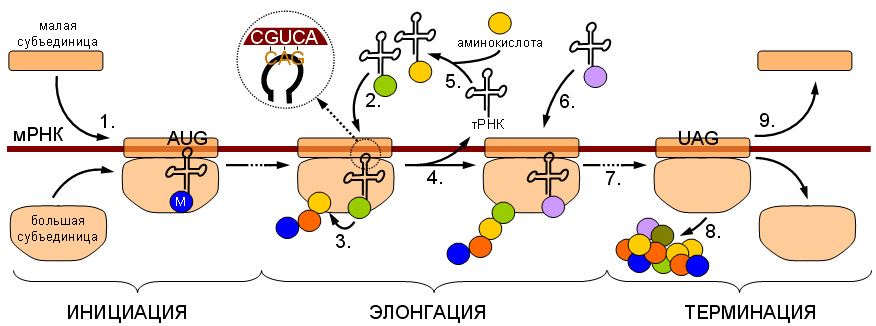
\includegraphics[width=0.8\textwidth]{Pictures/5_3(translation_e).jpg}
    \caption{Схема трансляции}
    \label{fig:5_3(translation_e)}
\end{figure}


\subsection{Структура рибосомы. Рибосомная РНК и белки}

\Def{Рибосома}(от «РНК» и soma – тело) -- клеточный немембранный\footnote{Немембранные органеллы лишены собственной замкнутой мембраны и не имеют четкой границы с цитоплазмой.} органоид, осуществляющий трансляцию (считывание кода мРНК и синтез полипептидов).  Присутствует у всех живых организмов, находится в жидкой внутренней среде клетки -- цитоплазме(рис. \ref{fig:5_1(cells)}). Состоит из рРНК(рибосомных РНК) и р-белков. 

По строению рибосома состоит из двух субъединиц: малой (1 молекула рРНК и 33 белка) и большой (3 молекулы рРНК и 40 белков), которые  соединяются вместе только на молекуле мРНК для синтеза белка. Малая субъединица считывает информацию с матричной РНК, а большая — присоединяет соответствующую аминокислоту к синтезируемой цепочке белка (рис. \ref{fig:5_24}). Массы субъединиц выражаются в измеряемых напрямую константах седиментации (скорость осаждения в единицах Сведберга, S)

\begin{figure}[h]
    \centering
    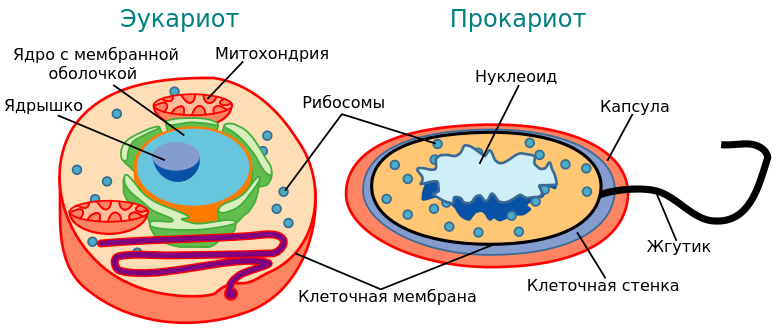
\includegraphics[width=0.7\textwidth]{Pictures/5_1(cell)}
    \caption{Строение клетки}
    \label{fig:5_1(cells)}
\end{figure}

Рибосомы в клетках эукариот состоят из четырех нитей РНК (три молекулы рРНК в большой субъединице и одна молекула рРНК – в малой) и примерно 80 разных белков, т.е представляют собой сложнейший комплекс из молекул, скрепленных слабыми, нековалентными связями. Рибосомы в клетках прокариот состоят из трех нитей РНК; две нити рРНК находятся в большой субъединице и одна рРНК – в малой. 

рРНК синтезируются РНК-полимеразой I в виде длинной молекулы пред-рибосомальной РНК, которая разрезается на отдельные РНК, составляющие основу рибосом.

\subsection{Функциональные активности и функциональные участки рибосомы}

Рибосома в процессе трансляции выполняет следующие функции:  

\begin{itemize}
    \item Связывание  и удержание  матричного полинуклеотида  (мРНК-связывающий участок)
    
    \item Удержание  пептидил-тРНК    или   деацилированной тРНК  (тРНК-связывающий  Р-участок);
    
    \item Связывание  аминоацил-тРНК  (тРНК-связывающий А-участок);
    
    \item Связывание  белковых  факторов  трансляции  и  ГТФ (факторсвязывающий  участок);
    
    \item Участие в катализе гидролиза ГТФ;
    
    \item Катализ транспептидации -- процесса, при котором аминокислота прикрепляется к хвосту уже собранного белка.
    
    \item Транслокация -- перемещение рибосомы по мРНК на один триплет.
\end{itemize}



\begin{figure}[h]
\begin{minipage}[h]{0.5\linewidth}
\center{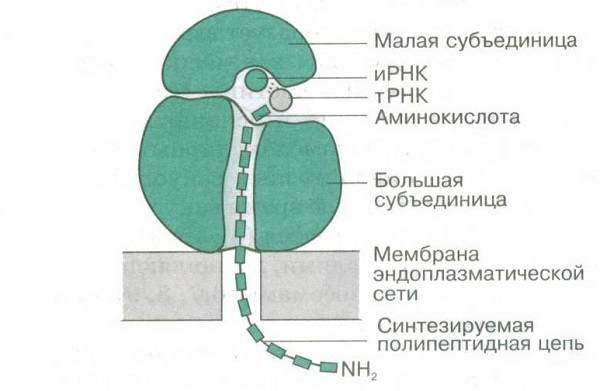
\includegraphics[width=0.7\linewidth]{Pictures/5_2(rybosome).jpg} \\ а)}
\end{minipage}
\hfill
\begin{minipage}[h]{0.5\linewidth}
\center{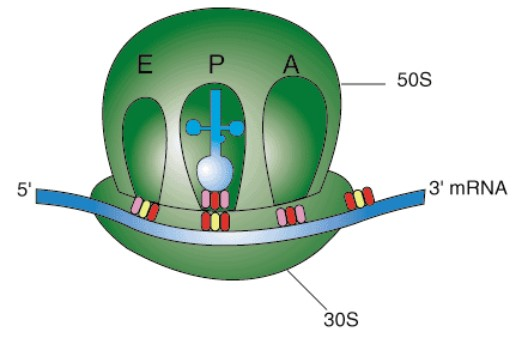
\includegraphics[width=0.6\linewidth]{Pictures/5_4(sites).jpg} \\ б)}
\end{minipage}
\caption{Строение рибосомы: а) расположение субъединиц б) расположение функциональных участков}
\label{fig:5_24}
\end{figure}


В процессе элонгации участие два белковых фактора. Первый переносит аминоацилированную («заряженную» аминокислотой) тРНК в А (аминоацил)-сайт рибосомы(рис. \ref{fig:5_24}б). Рибосома катализирует перенос пептида, связанного с тРНК в Р-сайте, в А-сайт и образование пептидной связи с находящимся там аминокислотным остатком(то есть тРНК "приносит" часть белка, а рибосома присоединяет его к строящейся цепочке). Таким образом растущий пептид удлиняется на один аминокислотный остаток. 

Затем второй белок катализирует транслокацию — перемещение рибосомы по мРНК на один триплет, в результате которого пептидил-тРНК оказывается вновь в Р-сайте, а «пустая» тРНК из P-сайта переходит в Е-сайт (от слова exit). тРНК из E-сайта диссоциирует спонтанно, после чего рибосома готова к новому циклу элонгации.

\subsection{Информационные и транспортные РНК. Аминоацил-тРНК-синетазы}

\Def{Информационная(=матричная) РНК}
Поскольку прокариотическая мРНК не нуждается в обработке и транспортировке, трансляция рибосомой может начаться немедленно после транскрипции. Следовательно, можно сказать, что трансляция у прокариот совмещена с транскрипцией и происходит ко-транскрипционно.

Эукариотическая мРНК должна быть обработана и доставлена из ядра в цитоплазму, и только тогда может быть транслирована рибосомой. Трансляция может происходить как на рибосомах, находящихся в цитоплазме в свободном виде, так и на рибосомах, ассоциированных со стенками эндоплазматического ретикулума. Таким образом, у эукариот трансляция не совмещена напрямую с транскрипцией. 

\Def{Транспортные РНК}
Одноцепочечная последовательность в форме листа клевера. Она формирует одноцепочечный участок, который заканчивается последовательностью ЦЦА со свободной ОН-группой. К этому концу присоединяется транспортируемая аминокислота. 3 остальные части представляют собой комплементарно спаренные последовательности нуклеотидов, которые заканчиваются неспаренными участками, образующими петли.

\Def{Аминоацил-тРНК-синетаза}
Транспортная тРНК(61 вид) и соответствующая ец аминокислотаа(20 видов) соединяются с помощью специального белка -- Аминоацил-тРНК-синетазы. Аминоацил = кислотный остаток, синтетаза = белок, синтезирующий что-то. К 3' концу тРНК прицепляется аминокислота и белок отделяется.

\subsection{Энергетика биосинтеза белка, использование АТФ и ГТФ}

Синтез белка -- энергозатратный процесс. Энергия на создание связи между тРНК и аминокислотой берется из гидролиза нуклеозидтрифосфатов АТФ и ГТФ.

Аминокислота активируется с использованием АТФ и присоединяется к тРНК с помощью фермента аминоацил-тРНК-синтетазы.

\Def{АТФ}
(Аденозинтрифосфат) -— нуклеозидтрифосфат.  

АТФ относится к так называемым макроэргическим соединениям, то есть к химическим соединениям, содержащим связи, при гидролизе которых происходит освобождение значительного количества энергии. Гидролиз макроэргических связей молекулы АТФ, сопровождаемый отщеплением 1 или 2 остатков фосфорной кислоты, приводит к выделению, по различным данным, от 40 до 60 кДж/моль. 

Подробнее в следующем разделе и на рис. \ref{fig:5_6(init_pro)}

\subsection{Инициация трансляции у прокариот, последовательность Шайна-Далгарно}


Первую фазу трансляции — инициацию — можно разделить на несколько стадий. На первой стадии два белковых фактора инициации IF-1 и IF-3 связываются с 30S-субчастицей (рис. \ref{fig:5_6(init_pro)}(1)). Затем еще один белковый фактор, IF-2, образует комплекс с ГТФ (GTP) (рис. \ref{fig:5_6(init_pro)}(2)), что облегчает ассоциацию 30S-субчастицы с мРНК (mRNA) и связывание тРНК (tRNA), соответствующей инициирующему кодону (рис. \ref{fig:5_6(init_pro)}(3)). У прокариот стартовая тРНК несет N-формилметионин (f-Met), у эукариот — метионин. В завершение 50S-субчастица связывается с вышеупомянутым комплексом (рис. \ref{fig:5_6(init_pro)}(4)). На третьей и четвертой стадиях идет освобождение факторов инициации и гидролиз связанного с IF-2 ГТФ до ГДФ (GDP) и неорганического фосфата Р. Таким образом, связанный с 70S-рибосомой инициирующий комплекс содержит формилметионин-тРНК в тРНК-связывающем участке, называемом пептидильным участком (Р). Второе место связывания, акцепторный участок (А), во время этой фазы трансляции остается свободным.

\begin{figure}[h]
    \centering
    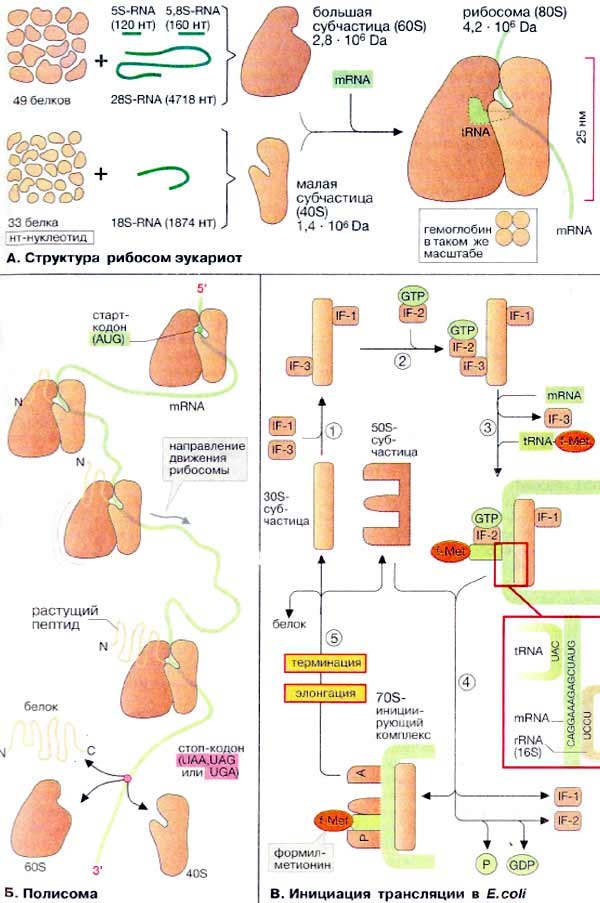
\includegraphics[width=0.5\textwidth]{Pictures/5_6(init_pro).jpg}
    \caption{Трансляция у прокариот на примере E.coli}
    \label{fig:5_6(init_pro)}
\end{figure}

\Def{Последовательность Шайна — Дальгарно} 
-- сайт связывания рибосом AGGAGG на молекуле мРНК прокариот, обычно на расстоянии около 10 нуклеотидов до стартового кодона AUG; в случае E. coli последовательность Шайна — Дальгарно — AGGAGGU. Комплементарная последовательность CCUCCU, называемая последовательностью анти-Шайна — Дальгарно, располагается на 3'-конце молекулы 16S рибосомной РНК. Комплементарное взаимодействие между последовательностями Шайна — Дальгарно и анти-Шайна — Дальгарно служит для помещения старт-кодона мРНК в P-сайт рибосомы для начала биосинтеза белка.

\subsubsection{Терминация трансляции прокариот}

Факторы терминации:

\begin{itemize}
    \item RF-1 вызывает отделение полипептидной цепи при считывании кодонов UAA и UAG;
    \item RF-2 действует аналогичным образом при считывании UAA и UGA;
    \item EF-3 может облегчить работу двух других факторов.
\end{itemize}

Этапы терминации трансляции прокариот:

\begin{itemize}
    \item В А-участке оказывается один из трех терминирующих кодонов –UAG, UAA или UGA;
    \item Из-за отсутствия тРНК, отвечающих этим кодонам,полипептидил-тРНКостается связанной с Р-участком RF-1 и RF-2 катализируют отсоединение полипептидной цепи от тРНК, отделение их обоих от рибосомы, а 70S-рибосомы –от мРНК;
    \item RF-1 узнает в А-участке кодон UAA или UAG•RF-2 включается в том случае, когда в А-участке оказывается UAA или UGA;
    \item RF-3 облегчает работу двух других факторов;
    \item Если терминирующим кодоном является UAA, то эффективность процесса терминацииоказывается наибольшей, поскольку этот кодон узнают оба фактора –RF-1 и RF-2.
\end{itemize}

\subsection{Инициация трансляции у эукариот, кэп-сайт.Терминация трансляции.}

Кэп представляет собой модифицированный рибонуклеотид — 7-метилгуанозин, соединённый 5'-трифосфатным мостиком с первым нуклеотидным остатком транскрипта. Кэп способствует эффективному процессингу пре-мРНК, экспорту мРНК из ядра, её трансляции и защите от быстрой деградации.

У эукариот старт-сайтом трансляции обычно (но не всегда) является AUG кодон.
Консенсусная последовательность Козак, играющая важную роль в инициации трансляции у эукариот, включает 4-6 нуклеотидов, предшествующих старт-кодону, и 1-2 нуклеотида непосредственно после старт-кодона. 

Оптимальный нуклеотидный контекст AUG кодона, коррелирует с высоким уровнем синтеза белка ссоответствующей мРНК in vivo и является характеристикой так называемой "сильной" (эффективно инициирующей трансляцию) последовательности Козак.

Последовательность Козак не является сайтом связывания рибосомы, в отличие от прокариотической последовательности Шайна-Дальгарно.

\begin{figure}[h]
    \centering
    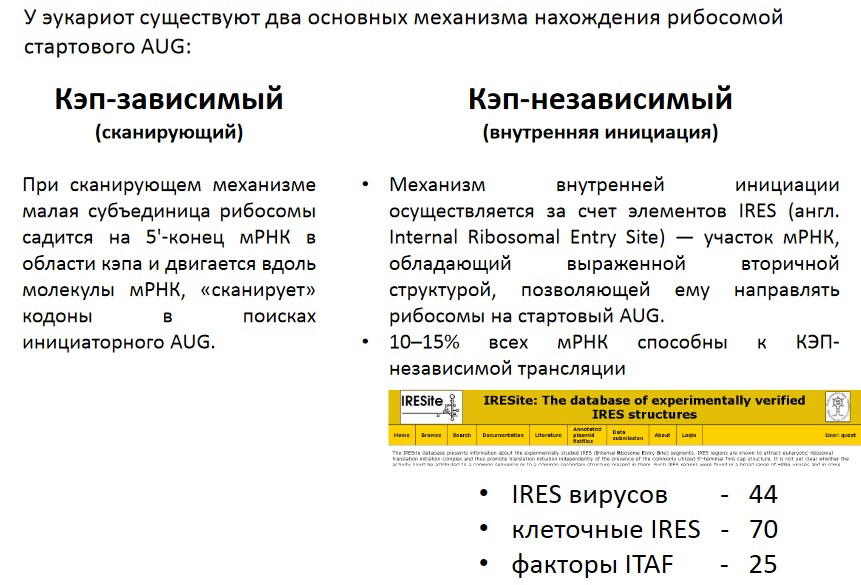
\includegraphics[width=0.7\textwidth]{Pictures/5_5(init_eu).jpg}
    \caption{Типы инициации трансляции эукариот}
    \label{fig:5_5(init_eu)}
\end{figure}

\subsubsection{Терминация трансляции эукариот}

Терминация происходит аналогично прокариотам. Терминация белкового синтеза у эукариот требует по крайней мере двух белков (eRF's от eukaryotic release factors), eRF1 и eRF3.